\newpage
\pagestyle{default}
\chapter{Introduction}
\thispagestyle{default}
Medical imaging plays a critical role in modern healthcare, supporting clinicians in diagnosing a wide range of conditions, from lung tumors to chest diseases and other life-threatening emergencies. As imaging technologies become more advanced and widely available, the volume of medical scans produced each day continues to grow. This rapid increase has intensified the need for efficient, reliable, and scalable diagnostic support systems that can assist healthcare professionals in interpreting complex visual data. \par

Recent advances in computer vision have made automated medical image analysis a promising tool for improving diagnostic accuracy and reducing clinical workload. Deep learning models, in particular, have demonstrated exceptional performance in tasks such as classification, localization, and segmentation across many imaging modalities. However, despite their capabilities, traditional centralized learning approaches often face critical limitations—especially in sensitive domains like healthcare, where data privacy, institutional policies, and regulatory constraints restrict the sharing of patient information. \par

To address these challenges, new paradigms in machine learning and model transparency have emerged. Federated learning enables collaborative training across multiple medical institutions without requiring direct access to patient data, offering a pathway toward more diverse and robust models while preserving privacy. Complementing this, explainable AI techniques provide insights into model decisions, helping clinicians understand why a prediction was made and increasing trust in AI-assisted diagnostics. \par

This project aims to integrate these three powerful components—computer vision, explainable AI, and federated learning—into a unified system designed to support medical image analysis across a variety of diseases and emergency conditions. By leveraging decentralized learning and transparent decision-making, the system seeks to improve accuracy, reliability, and interpretability while respecting the privacy and variability inherent in real-world clinical environments. \par

\section{Problem Definition}
\label{sec:problem_definition}

Accurate diagnosis, precise segmentation, and localized identification of multi-class thoracic pathologies from projectional radiography (X-ray) and cross-sectional computed tomography (CT) images remain a critical, life-saving bottleneck in contemporary emergency and clinical healthcare systems. In high-volume triage environments, intensive care units, and resource-constrained medical centers, clinicians and radiologists are subjected to immense cognitive fatigue, psychological stress, and severe time constraints. Under these taxing diagnostic conditions, many clinically critical anomalies can be visually subtle, transient, or easily obscured by surrounding dense anatomical architectures. 

For instance, early-stage alveolar consolidations, hidden or subpleural tuberculous granulomas, micro-nodular viral patterns, or tiny, solitary tumor-like pulmonary lesions are inherently faint and frequently masked by overlying  structures (such as the ribs, clavicles, and scapulae), complex central vascular configurations, or soft-tissue summation artifacts. Overlooking these fine radiological indicators can lead to severe diagnostic delays, inappropriate patient discharge, cross-infection risks in hospital wards, uncontrolled systemic disease progression, and significantly compromised long-term patient survival outcomes.

While modern deep learning architectures, particularly Convolutional Neural Networks (CNNs) and Vision Transformers (ViTs), have achieved state-of-the-art performance in isolated computer-aided diagnostic benchmarks, their meaningful clinical integration within hospital workflows remains profoundly limited by two overarching, systemic barriers:
\begin{enumerate}
	\item \textbf{Data Siloing, Fragmentation, and Strict Privacy Barriers:} Training a deep learning model capable of high generalization across diverse clinical settings requires massive, multi-institutional, and highly heterogeneous datasets. However, medical data is heavily siloed due to strict ethical, legal, and regulatory compliance standards enforced worldwide, such as the Health Insurance Portability and Accountability Act (HIPAA) in the United States and the General Data Protection Regulation (GDPR) in the European Union. Institutions are strictly prohibited from aggregating, uploading, or sharing raw patient imaging data to centralized cloud repositories or external computing hubs. Consequently, models trained on isolated, single-institution datasets suffer from severe overfitting and fail to generalize when deployed across external diagnostic setups or varying patient demographics.
	\item \textbf{The "Black-Box" Nature and Lack of Clinically Verifiable Interpretability:} Standard deep learning pipelines produce deterministic classification vectors or bounding coordinate values without generating clear, human-interpretable rationale for their decision-making. Medical practitioners cannot ethically, legally, or clinically trust automated diagnoses that lack transparent, physiological justification. If a model detects a malignancy or a highly infectious respiratory condition without visually mapping the corresponding lesion, patch, or parenchymal disruption, the clinician cannot easily verify, audit, or trust the output, limiting the artificial intelligence to a novelty tool rather than a viable diagnostic assistant.
\end{enumerate}

Furthermore, medical data exhibits severe Non-Identically and Independently Distributed (Non-IID) characteristics across disparate hospitals. Variations in imaging hardware manufacturers (e.g., GE, Siemens, Philips), localized X-ray tube voltages, exposure settings, slice thicknesses in CT imaging, patient demographics, regional disease prevalence, and distinct institutional positioning protocols introduce massive data distribution shifts. When institutional datasets are highly heterogeneous, standard centralized optimization functions collapse, leading to catastrophic forgetting or severe performance degradation for minority disease classes or specific imaging modalities.

Given this multi-faceted medical and technical challenge, the central problem addressed by this research is formally stated as follows:

\begin{quote}
	\textit{\textbf{How can we engineer an integrated, privacy-preserving, mathematically robust, and highly explainable deep learning framework capable of simultaneously detecting and localizing four major thoracic disease classes (pneumonia, tuberculosis, COVID-19, and tumor-like chest masses/lung cancer) using heterogeneous X-ray and CT image streams, without transmitting sensitive patient data beyond institutional boundaries, and while generating clinically verifiable visual explanations that clinicians can trust?}}
\end{quote}

To formalize this problem within a unified multi-modal diagnostic pipeline, the target diseases, structural anomalies, and their corresponding diagnostic modalities are defined below:

\begin{itemize}
	\item \textbf{Pneumonia (X-ray Modality):} An acute, inflammatory parenchymal lung infection causing fluid, pus, and cellular debris accumulation inside the alveoli. This condition manifests on chest radiographs as areas of increased opacity, visible as dense lobar consolidations, patchy bronchopneumonic infiltrates, or diffuse interstitial markings that obscure the underlying clear pulmonary margins.
	\item \textbf{Tuberculosis (TB) (X-ray/CT Modality):} A chronic, granulomatous infectious disease caused by \textit{Mycobacterium tuberculosis}. Radiographically, it exhibits a highly diverse presentation including apical fibro-nodular infiltrates, thick-walled cavitary lesions resulting from caseous tissue necrosis, hilar or mediastinal lymphadenopathy, or disseminated miliary micro-nodules distributed throughout the lung fields.
	\item \textbf{COVID-19 (X-ray Modality):} A highly infectious viral pneumonia caused by SARS-CoV-2. It presents with characteristic subpleural, peripheral, and basal ground-glass opacities (GGOs) that can progress rapidly into confluent, bilateral consolidations with extensive pulmonary involvement, creating acute ventilation-perfusion mismatching.
	\item \textbf{Chest Masses, Lung Cancer, and Tumor-like Abnormalities (CT Modality):} Neoplastic, space-occupying cellular proliferations within the lung parenchyma, mediastinum, or bronchial tree. Evaluated via high-resolution chest CT scans, these present as solid, sub-solid, or ground-glass solitary pulmonary nodules or large masses, characterized by malignant morphological signatures such as spiculation, lobulation, and eccentric calcification patterns.
	\item \textbf{Normal / Baseline Cases (Multi-Modal):} Thoracic imaging datasets exhibiting entirely pristine, healthy lung fields, intact vascular markings, and uncompromised pleural spaces, serving as the baseline control class for the multi-class objective function to prevent false positive classifications.
\end{itemize}

Successfully executing an automated system to address these conditions within a single unified framework introduces several technical, mathematical, and algorithmic challenges:

\begin{itemize}
	\item \textbf{Extreme Morphological Subtlety and Feature Overlap:} Many targeted pathologies exhibit overlapping visual characteristics. For instance, early-stage lung cancer can mimic a localized tuberculous granuloma on a CT scan, while viral pneumonia, atypical bacterial infections, and early COVID-19 can display identical ground-glass signatures on a chest radiograph. Models must capture fine-grained features to avoid cross-class misclassification.
	\item \textbf{Strict Regulatory, Legal, and Privacy Constraints:} The system must comply with zero-trust data architectures. Raw clinical DICOM files cannot be pooled or aggregated centrally, necessitating decentralized training algorithms where only abstract model parameters, localized weights, or gradient updates are shared over secure networks.
	\item \textbf{Statistical Heterogeneity (Non-IID Data Profiles):} The random partitioning of data across different clinical sites yields highly unbalanced label distributions (feature and label skewness). The framework must remain resilient against local client drift, preventing individual hospital nodes from skewing the global aggregated model optimization path.
	\item \textbf{Explainable Artificial Intelligence (XAI) Alignment:} The model must tightly couple its predictive classification heads with pixel-level attribution maps (such as Gradient-weighted Class Activation Mapping or Attention Maps). These visual explanations must pinpoint the exact diseased parenchymal region or mass boundary, mapping directly to recognized radiological signs.
	\item \textbf{Communication Efficiency and Deployment Constraints:} Transmitting heavy deep-learning model parameters across decentralized institutional nodes introduces severe bandwidth, latency, and communication overhead. The framework must utilize highly optimized architectures to enable real-world federated deployment across medical centers with varying network conditions.
\end{itemize}

To systematically overcome these challenges, this work designs, implements, and evaluates an integrated, enterprise-grade deep framework: \textit{X-Fed NeuroScan}. By synthesizing advanced edge-computed federated learning algorithms for privacy-preserving, collaborative multi-institutional model development with cutting-edge Explainable AI (XAI) pipelines, \textit{X-Fed NeuroScan} delivers highly accurate, safe, and transparent multi-class diagnostic outputs. This framework preserves patient data privacy by design while offering visual justifications that allow clinicians to confidently verify and act upon the model's findings.

\begin{table}[htbp]
	\centering
	\caption{Systemic problem matrix: Mapping technical challenges to the corresponding structural elements of the framework for thoracic disease detection.}
	\label{tab:problem_framework_matrix}
	\small
	\begin{tabularx}{\textwidth}{lXX}
		\toprule
		\textbf{Core Challenge Category} & \textbf{Radiological / Clinical Impact} & \textbf{Algorithmic Mitigations} \\
		\midrule
		\textbf{Visual Anomaly Subtlety} & Faint ground-glass patches or early masses are overlooked during clinical triage. & Advanced multi-scale feature extractors and high-resolution spatial processing pipelines. \\
		\addlinespace
		\textbf{Data Siloing \& Privacy} & Small institutional datasets limit model generalization and trigger model overfitting. & Decentralized federated learning protocol; raw patient data never leaves the local node. \\
		\addlinespace
		\textbf{Statistical Non-IID Skew} & Variations in scanner brands and local demographics degrade centralized optimization. & Weighted model aggregation strategies designed to stabilize decentralized parameter updates. \\
		\addlinespace
		\textbf{Opaque Decision-Making} & Clinicians reject AI classification due to an inability to audit or trust the underlying logic. & Deep XAI layer coupling that outputs spatial heatmaps corresponding to anatomical lesions. \\
		\bottomrule
	\end{tabularx}
\end{table}


\section{Challenges in Medical Image Analysis}

Medical imaging plays a fundamental role in modern healthcare, providing clinicians with valuable information for diagnosing, monitoring, and treating a wide range of diseases. Imaging modalities such as chest X-rays and Computed Tomography (CT) scans are routinely used to assess abnormalities within the thoracic region, including pneumonia, tuberculosis, pulmonary edema, and lung cancer. Despite the significant advancements in imaging technologies, the interpretation and analysis of medical images remain highly challenging tasks.

Medical image analysis traditionally relies on the expertise of radiologists and physicians who must examine large volumes of imaging data and identify subtle patterns that may indicate disease. The complexity of anatomical structures, variability among patients, and limitations of human perception can make accurate diagnosis difficult. These challenges can affect diagnostic accuracy, increase workload, and potentially delay clinical decision-making.

\subsection*{Complex Anatomical Structures}

The human thoracic cavity contains numerous overlapping anatomical structures, including the lungs, heart, ribs, blood vessels, diaphragm, and surrounding soft tissues. In chest X-ray images, these structures are projected onto a two-dimensional plane, causing different tissues to overlap and potentially obscure important pathological findings.

The presence of overlapping structures makes it difficult for clinicians to accurately distinguish between normal anatomical variations and disease-related abnormalities. Small lesions, nodules, or early-stage infections may be hidden behind ribs or other dense structures, increasing the likelihood of missed diagnoses.

\subsection*{Subtle Appearance of Early-Stage Diseases}

Many thoracic diseases initially manifest as subtle visual changes that are difficult to detect through routine examination. Early-stage lung cancer, for example, may appear as a small pulmonary nodule that is barely distinguishable from surrounding tissue. Similarly, mild pneumonia or early tuberculosis infections may produce only faint abnormalities within the lung fields.

Detecting these subtle findings requires significant expertise and experience. Even highly trained radiologists may encounter difficulties when abnormalities are small, poorly defined, or located in anatomically complex regions.

\subsection*{Variability in Disease Presentation}

The same disease can appear differently across patients due to factors such as age, disease stage, genetic characteristics, and the presence of other medical conditions. Furthermore, different diseases may exhibit similar radiological appearances, making differential diagnosis challenging.

For example, pulmonary infections, inflammatory conditions, and certain types of lung cancer can produce similar opacities in chest X-rays. Likewise, benign and malignant lung nodules may share similar characteristics in CT scans. This variability increases diagnostic complexity and may lead to uncertainty during image interpretation.

\subsection*{Dependence on Radiologist Expertise}

Accurate medical image interpretation requires extensive education, training, and clinical experience. Radiologists must possess detailed knowledge of anatomy, pathology, imaging physics, and disease progression in order to make reliable assessments.

However, diagnostic performance can vary among clinicians depending on their level of expertise and familiarity with specific conditions. Less experienced practitioners may overlook subtle findings or misinterpret complex cases. As a result, diagnostic consistency can differ between healthcare professionals and institutions.

\subsection*{Inter-Observer and Intra-Observer Variability}

One of the well-known challenges in medical imaging is the variability in interpretation among radiologists. Different specialists may provide different assessments when evaluating the same image, a phenomenon known as inter-observer variability.

Additionally, the same radiologist may occasionally reach different conclusions when reviewing an image at different times, which is referred to as intra-observer variability. Such inconsistencies can affect diagnostic reliability and complicate treatment planning, particularly in borderline or ambiguous cases.

\subsection*{Large Volume of Imaging Data}

Modern healthcare systems generate enormous quantities of medical images on a daily basis. Radiologists are often required to review hundreds of imaging studies during a single workday, creating significant workload pressures.

CT examinations present an additional challenge because a single scan may contain hundreds of image slices that must be carefully reviewed. Thorough examination of such large datasets is time-consuming and can contribute to fatigue, potentially increasing the risk of oversight or diagnostic errors.

\subsection*{Time Constraints in Clinical Practice}

Healthcare professionals frequently operate under strict time constraints, particularly in busy hospitals and emergency departments. Rapid diagnosis is often essential for initiating timely treatment and improving patient outcomes.

The need to balance speed with diagnostic accuracy can be challenging, especially when dealing with complex imaging studies. Under time pressure, subtle abnormalities may be overlooked, and difficult cases may require additional consultation or follow-up examinations.

\subsection*{Image Quality Limitations}

The diagnostic quality of medical images can be affected by several factors, including patient movement, improper positioning, low contrast, imaging noise, and equipment-related artifacts. Poor image quality may obscure important pathological findings and make interpretation more difficult.

In chest X-ray imaging, underexposure or overexposure can reduce visibility of anatomical details. In CT imaging, motion artifacts caused by breathing or patient movement can degrade image clarity. Such limitations may reduce diagnostic confidence and necessitate repeat imaging procedures.

\subsection*{Diagnostic Errors and Missed Findings}

Despite advances in medical imaging technology, diagnostic errors remain an unavoidable challenge. Errors may occur due to perceptual limitations, cognitive biases, fatigue, distraction, or the inherently complex nature of certain cases.

Missed lung nodules, overlooked fractures, and undetected early-stage diseases represent some of the most common diagnostic challenges in thoracic imaging. Because delayed diagnosis can significantly impact patient outcomes, minimizing such errors remains a major objective within radiology.

\subsection*{Challenges in Lung Cancer Detection}

Lung cancer detection presents particularly significant difficulties due to the diverse appearance of pulmonary nodules. Nodules may vary greatly in size, shape, texture, density, and location. Small malignant nodules can closely resemble benign lesions or normal anatomical structures.

Furthermore, certain tumors may be partially obscured by blood vessels, ribs, or surrounding tissues. Accurate identification and characterization of suspicious nodules often require careful examination across multiple CT slices and comparison with previous studies, making the diagnostic process both complex and time-intensive.

\subsection*{Increasing Demand for Radiological Services}

The global demand for medical imaging services continues to grow due to population growth, aging demographics, and increased utilization of diagnostic imaging technologies. However, many healthcare systems face shortages of trained radiologists and imaging specialists.

This imbalance between demand and available expertise can lead to increased workloads, longer reporting times, and reduced access to timely diagnoses. The challenge is particularly pronounced in developing regions and underserved healthcare environments.


\section{Background and Motivation}
The rapid growth of medical imaging data, coupled with increased clinical workloads, has made conventional diagnostic workflows increasingly insufficient. Although automated analysis using computer vision holds considerable promise in improving diagnostic accuracy and efficiency, practical implementation is hindered by challenges such as patient privacy restrictions, limited data set diversity, and substantial computational and data transfer demands. Therefore, a thorough understanding of both the potential benefits and inherent limitations of AI in medical imaging is essential for the design of systems that are accurate, interpretable, and scalable in heterogeneous clinical environments.
\subsection*{Rise of Computer Vision in Automated Analysis}

The rapid digitization of healthcare has led to a dramatic increase in medical imaging data, including X-ray, CT, MRI, and ultrasound scans. Radiologists now face the dual challenges of handling large patient loads and interpreting large volumes of images quickly and accurately. Computer vision has emerged as a crucial tool for addressing these demands by enhancing diagnostic efficiency and accuracy.

To understand why computer vision is now widely adopted in clinical workflows, consider the following advantages:

\begin{itemize}
	\item \textbf{High sensitivity to subtle patterns}: AI can detect faint fractures or early-stage tumors.
	\item \textbf{Rapid processing}: Thousands of images can be analyzed within seconds.
	\item \textbf{Consistency}: Predictions remain stable regardless of fatigue or emotional state.
	\item \textbf{Adaptability}: Deep models can generalize to various imaging modalities.
\end{itemize}

The effectiveness of computer vision in medical imaging is reinforced by major achievements in the field. These advancements primarily arise from deep learning architectures such as CNNs and Vision Transformers. In practice, computer vision supports several core tasks:

\begin{enumerate}
	\item Classification of abnormal vs. normal scans.
	\item Localization of suspicious areas using object detection.
	\item Segmentation of organs, lesions, and fracture regions.
	\item Identification of patterns that deviate from healthy anatomy.
\end{enumerate}

A concise summary of computer vision benefits in medical imaging is outlined in Table~\ref{tab:cv_roles}.

\vspace{0.3cm}

\begin{table}[h!]
	\centering
	\renewcommand{\arraystretch}{1.3}
	\setlength{\tabcolsep}{10pt}
	
	\caption{\small Key Advantages of Computer Vision in Medical Image Automation}
	\label{tab:cv_roles}
	
	
	\begin{tabular}{|p{5cm} | p{8cm}|}
		\hline
		{\textbf{Computer Vision Capability}} &
		{\textbf{Role in Medical Imaging}} \\
		\hline
		
		Feature extraction &
		Detects subtle abnormalities beyond human perception \\
		\hline
		
		Automation of routine tasks &
		Reduces workload and radiologist fatigue \\
		\hline
		
		High-speed inference &
		Enables rapid triage in emergencies \\
		\hline
		
		Generalization across cases &
		Handles variations in anatomy and imaging conditions \\
		\hline
	\end{tabular}
\end{table}



\subsection*{Limitations of Centralized Machine Learning}

Despite the promise of AI-based diagnostic systems, models trained in a centralized manner face several constraints. These limitations arise mainly from restrictions on data availability, data diversity, and practical constraints in medical settings.

Centralized learning typically suffers from:

\begin{itemize}
	\item \textbf{Restricted data sharing}: Patient data cannot be freely exchanged due to privacy laws.
	\item \textbf{Lack of representation}: Single-hospital datasets fail to capture global patient diversity.
	\item \textbf{High storage and transfer requirements}: Medical images are large and expensive to move.
	\item \textbf{Data imbalance}: Rare conditions remain underrepresented, harming model performance.
\end{itemize}

These issues do not simply degrade model accuracy—they introduce significant risks into clinical AI deployment. The consequences can be better understood through the following observations:

\begin{enumerate}
	\item Models trained in isolation often misclassify images from new machines or demographics.
	\item Performance can fluctuate between institutions due to imaging protocol differences.
	\item Bias can emerge when the training set fails to include certain patient groups.
\end{enumerate}

Table~\ref{tab:centralization_challenges} summarizes these core limitations in a structured manner.

\vspace{0.3cm}

\begin{table}[h!]
	\centering
	\renewcommand{\arraystretch}{1.3}
	\setlength{\tabcolsep}{10pt}
	
	\caption{\small Challenges of Centralized Machine Learning in Healthcare}
	\label{tab:centralization_challenges}
	
	
	\begin{tabular}{|p{5cm} | p{8cm}|}
		\hline
		{\textbf{Limitation}} &
		{\textbf{Impact}} \\
		\hline
		
		Privacy restrictions &
		Prevent hospitals from sharing sensitive patient data \\
		\hline
		Limited dataset diversity &
		Reduces generalization to different populations or imaging devices \\
		\hline
		Large data transfer requirements &
		Increases cost and delays in model development \\
		\hline
		Imbalanced condition frequency &
		Degrades performance on rare diseases or subtle abnormalities \\
		\hline
	\end{tabular}
\end{table}

Centralized machine learning, while powerful, therefore struggles to meet the scalability, diversity, and privacy needs of real-world medical AI deployment. These challenges motivate the development of more robust learning paradigms capable of overcoming data fragmentation and institutional isolation.

\section{Suggested Solution}

The challenges identified in the medical imaging domain—including subtle abnormalities, limited dataset diversity, privacy constraints, and variability in imaging standards—necessitate a more advanced diagnostic support system. The proposed project aims to address these limitations by integrating three complementary technologies: Computer Vision, Explainable AI, and Federated Learning. Together, these components form an intelligent system capable of assisting clinicians in identifying fractures, tumors, infections, and other abnormalities more reliably and transparently.

The core idea behind the project is to design a computer vision pipeline capable of analyzing X-ray and other medical imaging modalities with high accuracy. Deep learning models will detect patterns that may be difficult for clinicians to recognize quickly, especially in emergency or high-stress situations. By augmenting image interpretation with AI-based classification and region highlighting, the system serves as a powerful second-opinion tool, reducing oversight and improving diagnostic confidence.

To ensure that the system remains trustworthy and clinically interpretable, Explainable AI techniques are incorporated to reveal how the model arrives at its predictions. This transparency allows medical professionals to understand the rationale behind the AI’s outputs, compare them with clinical knowledge, and detect any mistakes or biases early.

Moreover, Federated Learning is utilized to overcome the limitations of centralized training. Instead of pooling patient data into a single server—a process that is often legally and ethically restricted—hospitals collaboratively train the model without exposing sensitive information. This approach significantly increases dataset diversity while maintaining strict compliance with privacy regulations.

In summary, the proposed solution seeks to:

\begin{itemize}
	\item Improve diagnostic accuracy through advanced computer vision algorithms.
	\item Increase clinician trust via transparent and interpretable model outputs.
	\item Overcome data-sharing barriers by enabling collaborative, privacy-preserving training.
\end{itemize}

These three components work together to form a robust, scalable, and clinically meaningful AI-based diagnostic support framework.



\subsection*{Explainable Artificial Intelligence (XAI) in Thoracic Diagnostics}
\label{subsec:explainable_ai}

Explainable Artificial Intelligence (XAI) encompasses a robust suite of mathematical formulations, post-hoc algorithmic frameworks, and intrinsic architectural designs engineered to systematically dismantle the "black-box" paradigm of deep neural networks. By transforming opaque, multi-layered statistical representations into highly transparent, human-interpretable, and clinically auditable insights, XAI bridges the gap between advanced deep learning and clinical practice. 

As deep learning models grow exponentially in depth and structural complexity—leveraging billions of abstract parameters across dense convolutional layers or self-attention blocks—their internal latent spaces become completely divorced from standard human logic. In safety-critical fields like thoracic oncology and pulmonology, where an algorithmic failure can lead to catastrophic diagnostic errors, this lack of transparency presents a significant barrier to clinical adoption. XAI methods resolve this issue by providing verifiable visual or textual justifications that explain how and why an algorithm arrived at a specific diagnostic conclusion.

Within the specific domain of multi-class thoracic imaging (encompassing complex pathologies like pneumonia, COVID-19, tuberculosis, and lung cancer), explainability shifts from a theoretical asset to a strict clinical, ethical, and legal necessity. Rather than operating as a binary oracle that simply outputs a classification vector or a bounding box coordinates, an advanced explainable system maps its final prediction to specific, localized pixel-level features. These visual justifications allow radiologists and treating physicians to evaluate the physiological validity of the model's outputs. This capability serves as a vital confirmatory layer during high-stress triage workflows and protects against catastrophic false positives or negatives.

XAI supports and enhances clinical decision-making through several key mechanisms:

\begin{itemize}
	\item \textbf{High-Precision Spatial Localization:} Identifying and mapping the exact spatial coordinates, pixel boundaries, or macro-anatomical lung segments that drove the model's objective function toward a specific classification.
	\item \textbf{Spurious Feature Disconnection and Artifact Auditing:} Enabling developers and clinicians to verify that the network is optimization-grounded in genuine, peer-reviewed pathological markers (e.g., spiculation, ground-glass opacities, or cavitary walls) rather than over-indexing on irrelevant artifacts, such as digital scanner text, patient positioning markers, rib contours, or random background noise.
	\item \textbf{Algorithmic Error Detection and Bias Mitigation:} Facilitating the systematic detection of hidden model vulnerabilities, such as shortcut learning, distribution shifts, severe dataset bias, or systemic misinterpretations of normal structural variants (e.g., vascular bifurcations mistaken for micro-nodules).
	\item \textbf{Interactive Clinical Cross-Examination:} Providing a transparent visual baseline that empowers clinicians to confidently verify, critique, or override automated AI predictions by applying their extensive domain expertise and real-world experience.
	\item \textbf{Medico-Legal Compliance and Auditability:} Generating a clear, deterministic trail of visual evidence for every diagnostic output. This documentation satisfies rigorous regulatory standards, fits seamlessly into institutional electronic health records (EHR), and can be effectively communicated in patient-facing clinical reports.
\end{itemize}

A wide array of XAI methodologies are utilized across modern deep thoracic diagnostics, categorized primarily into gradient-based post-hoc attributions and intrinsic attention mechanisms. Linear and non-linear pixel-level saliency maps compute the direct gradients of the output score with respect to the input image, capturing highly granular sensitivity profiles. To provide cleaner, structurally localized visualizations, advanced frameworks leverage Class Activation Mapping (CAM) and Gradient-weighted Class Activation Mapping (Grad-CAM). These techniques tap into the final convolutional layers of a network to capture coarse semantic features and project them back onto the input image as heatmaps. 

Furthermore, with the introduction of Vision Transformers (ViTs) in medical imaging, attention-based visualization frameworks (such as Rollout or Value-Decomposition Attention) directly extract the internal self-attention matrix weights. This generates highly accurate heatmaps that reflect the global context and long-range structural dependencies learned by the network. Beyond pure spatial heatmaps, modern XAI pipelines also incorporate quantitative feature attribution scores, concept-based explanations, and automated natural-language diagnostic text generation. These advanced techniques map directly onto standard radiological vocabularies, ensuring that the model's reasoning aligns with established clinical workflows. Figure~\ref{fig:xai_in_action} illustrates the conceptual integration of an explainability layer within an automated diagnostic pipeline, highlighting how opaque latent representations are translated into interpretable spatial heatmaps.

\begin{figure}[H]
	\centering
	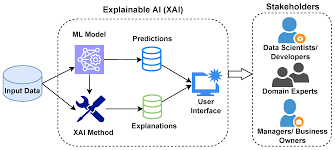
\includegraphics[width=0.65\linewidth]{assets/XAI.png}
	\caption{Explainable AI (XAI) layer integration within the automated diagnostic pipeline, illustrating the mapping of latent feature spaces to localized spatial heatmaps for clinical validation.}
	\label{fig:xai_in_action}
\end{figure}


\subsection*{Federated Learning Frameworks for Decentralized Thoracic Imaging}
\label{subsec:federated_learning}

Federated Learning (FL) represents a transformative decentralized optimization paradigm designed to facilitate collaborative, multi-institutional machine learning model development while guaranteeing complete local data sovereignty. In classical centralized deep learning frameworks, large-scale medical imaging repositories must be aggregated from multiple disparate clinical sites into a singular, central cloud repository or a unified computing infrastructure. This centralized architectural model introduces massive single-point-of-failure vulnerabilities, extreme network bandwidth consumption, and significant regulatory hurdles. 

Conversely, Federated Learning reverses this computational direction: rather than transmitting immense quantities of sensitive diagnostic imaging data over external networks to the centralized model, the abstract global model is transmitted directly to the decentralized institutional edge nodes. This foundational shift directly addresses the most critical hurdles in contemporary healthcare ecosystems, including strict patient privacy requirements, enterprise-grade data security protocols, legal liabilities, and the massive logistical burdens of cross-border medical dataset aggregation.

Within the high-stakes domain of clinical thoracic AI, datasets acquired across a multitude of independent hospitals, imaging centers, and regional health systems are fundamentally heterogeneous, geographically isolated, and legally protected[cite: 7, 10, 41]. Regulatory bodies enforce strict privacy statutes—such as the General Data Protection Regulation (GDPR) in the European Union and the Health Insurance Portability and Accountability Act (HIPAA) in the United States—which treat medical images and their associated metadata as highly sensitive Protected Health Information (PHI). 

Federated Learning provides a mathematically sound solution to these constraints by ensuring that raw patient data remains isolated behind institutional firewall structures throughout the entire lifecycle of model optimization[cite: 46]. The global model undergoes iterative optimization cycles by distributing parameter weights to individual clients, executing localized stochastic gradient descent loops entirely on edge hardware, and transmitting only abstract weight deltas or gradient updates back to a central orchestrating server. This collaborative process enables the underlying network to learn from massive, multi-institutional datasets of diverse patient distributions and varying scanner hardware configurations, which is critical for building a highly generalizable model capable of detecting rare, subtle lung abnormalities.

Federated Learning enhances clinical artificial intelligence development through several mechanisms:

\begin{itemize}
	\item \textbf{Complete Prevention of PHI Transmission:} Allowing diverse diagnostic centers to collaboratively train advanced deep networks without exposing, transmitting, or consolidating raw patient data.
	\item \textbf{Massive Global Generalizability and Scale:} Leveraging diverse datasets from distinct global populations, distinct geographic regions, and varying demographic slices, which directly prevents over-indexing on localized institutional distribution skews.
	\item \textbf{Significant Reduction of Data Breach Surfaces:} Mitigating systemic data breach risks and cyber-attacks by eliminating central honey-pot storage architectures, keeping sensitive information protected within local server environments.
	\item \textbf{Inherent Regulatory and Ethical Compliance:} Providing built-in compliance with evolving legal frameworks and data retention policies by minimizing data duplication and movement.
	\item \textbf{Continuous Edge-Driven Model Evolution:} Supporting lifelong and continuous learning patterns as edge institutions acquire new clinical imaging data during daily diagnostic workflows, without disrupting local institutional pipelines.
\end{itemize}

A multitude of aggregation strategies and architectural frameworks have been engineered to navigate the complex constraints of distributed medical imaging data. The foundational optimization baseline is \textit{Federated Averaging (FedAvg)}, where the central server initializes global model weights, distributes them to selected clients, and then computes a coordinate-wise weighted average of the local parameters based on the specific volume of data hosted at each institutional node after local optimization rounds. 

To stabilize convergence when dealing with severe non-IID client distributions, advanced aggregation algorithms like FedProx introduce proximal regularization terms to bound local parameter drift, while SCAFFOLD uses control variates to correct for localized client gradients. Furthermore, modern healthcare deployments implement security layers like Secure Aggregation (SecAgg) protocols based on cryptographic multi-party computation, alongside Differential Privacy (DP) techniques that add calibrated noise to local weight vectors to defend against reverse-engineering or model-inversion attacks. These privacy-preserving frameworks can also be paired with deep transfer learning, multi-task heads, and multi-modal feature fusion layers, allowing deep networks to optimize across distributed data streams while maintaining strong privacy guarantees. Figure~\ref{fig:federated_learning_pipeline} details the central-server approach to federated learning, illustrating the iterative parameter exchange loop between the global aggregator and the secure edge nodes.

\begin{figure}[H]
	\centering
	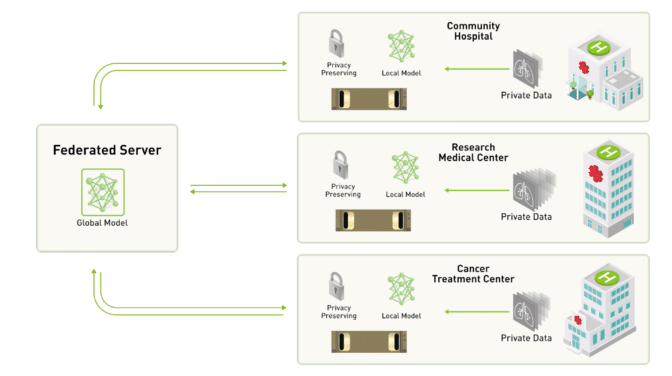
\includegraphics[width=0.8\linewidth]{assets/federated_learning.png}
	\caption{Centralized server architecture for federated learning, detailing the secure, iterative parameters exchange loop between the global orchestrator and localized institutional edge nodes.}
	\label{fig:federated_learning_pipeline}
\end{figure}

\section{Project Scope}
\label{sec:project_scope}

The fundamental scope of this research and development initiative centers on engineering, validating, and establishing an enterprise-grade, decentralized, and highly explainable medical computer vision ecosystem dedicated exclusively to multi-class thoracic pathology diagnosis. This advanced platform is structurally and algorithmically optimized to detect, classify, and spatio-temporally localize four highly prevalent, clinically severe, and socio-economically impactful thoracic conditions: acute pneumonia, Coronavirus Disease 2019 (COVID-19), chronic pulmonary tuberculosis (TB), and malignant lung cancer/chest masses. These conditions were strategically selected due to their massive contribution to global respiratory morbidity and mortality, the high risk of catastrophic clinical consequences if their initial radiological presentation is overlooked, and the immense structural variability they present across projectional and cross-sectional medical imaging modalities. By synthesizing advanced deep neural architectures with zero-trust decentralized optimization frameworks and post-hoc visual attribution models, this project scope explicitly establishes a robust, privacy-preserving machine learning diagnostic engine that can operate seamlessly across multi-institutional hospital networks.

The core technical boundary of this project is strictly defined by the integration, training, and fine-tuning of multi-modal deep learning models engineered to process two distinct clinical imaging streams. For the detection and differentiation of acute inflammatory and viral respiratory conditions (pneumonia and COVID-19), the system utilizes high-resolution projectional Chest X-ray (CXR) DICOM datasets, capturing fine-grained variations in alveolar and interstitial attenuation. For chronic infectious diseases and neoplastic lesions (tuberculosis, dense pulmonary masses, and lung cancer), the analytical pipeline is expanded to ingest and process high-contrast, cross-sectional chest Computed Tomography (CT) scans, enabling the extraction of multi-planar spatial features, volumetric nodule boundaries, and subtle morphological variations like edge spiculation or irregular calcifications. The machine learning pipeline is mathematically optimized to balance the trade-offs between diagnostic sensitivity and specificity, guaranteeing high recall to minimize false negative outcomes in clinical triage while maintaining precision to prevent downstream diagnostic bottlenecks and patient anxiety.

To guarantee seamless real-world deployability, abstract technological feasibility, and practical utility within active clinical environments, the backend diagnostic engine is natively wrapped inside a secure, low-latency, and web-based enterprise application interface. This front-end medical console is architected to allow non-technical healthcare practitioners, including front-line triage nurses, general physicians, emergency room technicians, and specialized thoracic radiologists, to securely ingest imaging files, execute distributed inference pipelines, and interact dynamically with the localized diagnostic outputs without requiring prior knowledge of deep learning mechanics, server configurations, or parameter tuning. While this cross-platform interface serves as a critical component for simulating real-world medical deployment and validating clinical integration, the primary focus, computational allocation, and academic scope of this project remain rigorously fixed upon the underlying mathematical formulations, decentralized federated optimization trajectories, model convergence stability under non-IID conditions, and the quantitative reliability of the explainable AI visualizations.

The functional boundaries and high-level architectural mandates of the system are categorized across four distinct, integrated operational vectors:

\begin{itemize}
	\item \textbf{Automated Multi-Class Thoracic Disease Identification:} Seamlessly processing heterogenous, multi-modal clinical image streams to perform differential classification across pneumonia, COVID-19, tuberculosis, and lung cancer/chest masses, effectively separating them from pristine normal baseline images.
	\item \textbf{Decentralized, Privacy-Preserving Collaborative Optimization:} Executing a secure, zero-trust federated learning protocol that orchestrates iterative parameter aggregation loops across distributed edge servers, strictly ensuring that protected health information (PHI) and raw patient images never exit local institutional firewalls.
	\item \textbf{Explainable Spatial Localization and Visual Justification:} Automatically coupling all deterministic classification outputs with high-fidelity, pixel-level attribution maps and self-attention weight heatmaps, explicitly highlighting the exact anatomical contours, parenchymal patches, or nodular boundaries that informed the network's predictive pathways.
	\item \textbf{Enterprise Web Deployment and Ingestion Architecture:} Constructing a secure web console featuring automated DICOM processing, smooth scaling across diverse hardware devices, and clean data visualizations tailored to match active clinical triage environments.
\end{itemize}

Crucially, the scope of this project is strictly defined by an assistive, clinician-in-the-loop operational philosophy and does \emph{not}, under any circumstances, aim to replace or supersede the definitive diagnostic judgment, clinical intuition, or legal accountability of professional medical practitioners or board-certified radiologists. Instead, the framework is meticulously engineered to function as an advanced, high-throughput second-opinion mechanism and triage assistant capable of reducing diagnostic oversights, mitigating human cognitive fatigue, and accelerating clinical turnaround times in high-volume emergency environments. 

Several technical boundaries are explicitly designated as out-of-scope for the current implementation phase to ensure absolute focus on the core machine learning and federated optimization objectives. The system is constrained to the four specified target conditions; the inclusion of other diffuse thoracic abnormalities (such as pneumothorax, chronic obstructive pulmonary disease, emphysema, or pleural effusions) falls entirely outside the project's current boundaries. Furthermore, while the federated learning layer is mathematically modeled and simulated to replicate a multi-hospital clinical network with severe statistical non-IID data distributions, the deployment scope is executed within distributed, multi-GPU simulated edge clusters rather than active, live-production hospital server backbones. Real-world institutional deployment across live physical hospital networks, real-time edge streaming, and expansion to handle non-thoracic disease modalities are deferred to future operational iterations, serving as logical continuations of this foundational architectural framework.

\begin{table}[htbp]
	\centering
	\caption{Project scope boundary matrix: Delineating technical inclusions, explicit exclusions, and target clinical metrics.}
	\label{tab:project_scope_matrix}
	\small
	\begin{tabularx}{\textwidth}{lXX}
		\toprule
		\textbf{Scope Category} & \textbf{Explicit Technical Inclusions} & \textbf{Explicit Technical Exclusions} \\
		\midrule
		\textbf{Target Pathologies} & Pneumonia, COVID-19, Pulmonary Tuberculosis (TB), and Lung Cancer/Chest Masses. & Pneumothorax, Emphysema, Pleural Effusions, Scoliosis, and Lung Nodules. \\
		\addlinespace
		\textbf{Imaging Modalities} & High-resolution projectional Chest X-rays (CXR) and cross-sectional chest CT scans. & Magnetic Resonance Imaging (MRI), Ultrasound, and Positron Emission Tomography (PET). \\
		\addlinespace
		\textbf{Data Protocols} & Zero-trust Federated Learning (FedAvg) using simulated non-IID distributed edge clients. & Live central cloud data pooling or live physical network integration into active EHR backbones. \\
		\addlinespace
		\textbf{Interpretability Layer} & Post-hoc visual attributions via Grad-CAM and self-attention rollout maps. & Automated clinical prescription generation or natural language therapy recommendations. \\
		\bottomrule
	\end{tabularx}
\end{table}

\section{Project Objectives} \label{sec:objectives}

The objectives of this project are centered around creating a reliable, accurate, and accessible diagnostic support system for lung tumor and chest diseases identification. The project aims to ensure that the system not only performs well in terms of machine learning metrics but also provides practical value to clinicians through usability, efficiency, and cost-effectiveness. Achieving clinical-level performance requires a well-defined set of goals that align both with technical constraints and real-world medical needs.

A primary objective is to develop a computer vision model capable of achieving high diagnostic performance. In particular, the system is designed to reach an accuracy above 90\% across its targeted conditions while maintaining a recall rate that minimizes the risk of missed fractures or tumors. Since false negatives can lead to severe clinical consequences, optimizing recall is essential for ensuring the safety and reliability of the system.

In addition to predictive performance, another major objective is to deliver an intuitive and engaging web interface that enables medical personnel to interact with the system easily. The interface should allow users to upload images, view results, and interpret highlighted regions without requiring technical expertise. Ease of use is critical for facilitating adoption in real clinical workflows, where time efficiency and clarity are important.

Operational efficiency is also a key objective. The system must be designed in a manner that minimizes computational overhead and reduces ongoing costs. This includes optimizing model size, using lightweight inference strategies where possible, and ensuring that the web application remains responsive even with limited hardware resources.

To summarize, the project seeks to meet the following objectives:

\begin{itemize}
	\item Achieve a diagnostic accuracy exceeding 90\% on lung tumor and chest diseases detection tasks.
	\item Maintain a high recall rate to reduce the likelihood of missed abnormalities.
	\item Provide a user-friendly, accessible, and engaging web interface suitable for non-technical clinical staff.
	\item Develop an efficient system that minimizes operational and computational costs.
\end{itemize}

Collectively, these objectives define the criteria by which the success of the project will be evaluated and guide the design decisions throughout development.

\section{Project Challenges}

Despite the remarkable progress achieved in recent years, medical image analysis remains a challenging field. The complexity of medical data, the critical nature of clinical decision-making, and the variability of imaging procedures introduce numerous obstacles that must be addressed to develop reliable and clinically applicable systems. The following subsections discuss the major challenges associated with medical image analysis, particularly in the context of chest disease detection using X-ray images and lung cancer detection using CT scans.

\subsection*{Limited Availability of High-Quality Medical Data}

One of the most significant challenges in medical image analysis is the limited availability of large, high-quality, and well-annotated datasets. Deep learning models generally require substantial amounts of labeled data to achieve high performance and robust generalization. However, obtaining medical images with accurate annotations is often difficult and expensive.

Medical image annotation requires the expertise of trained radiologists or medical specialists who must carefully examine each image and identify pathological findings. This process is time-consuming and resource-intensive. Furthermore, patient privacy regulations and ethical considerations often restrict the sharing of medical data between healthcare institutions, limiting the availability of publicly accessible datasets.

In the context of chest X-ray analysis, some diseases may occur infrequently, leading to severe class imbalance within datasets. Similarly, for lung cancer detection from CT scans, obtaining sufficiently large collections of confirmed malignant and benign cases can be challenging. These limitations can negatively affect model training and reduce diagnostic performance.

\subsection*{Variability in Image Acquisition}

Medical images are acquired using different imaging devices, protocols, and settings across hospitals and healthcare facilities. As a result, images may exhibit significant variations in quality, resolution, contrast, brightness, noise levels, and anatomical positioning.

Chest X-ray images obtained from different institutions may vary due to differences in machine manufacturers, patient positioning techniques, exposure settings, and image preprocessing procedures. Likewise, CT scans may differ in slice thickness, reconstruction algorithms, scanning protocols, and radiation dose levels.

Such variability can lead to distribution shifts between training and deployment environments. A model trained on data from one institution may experience performance degradation when applied to images acquired in another clinical setting. Ensuring robustness across diverse imaging conditions remains a major challenge for medical image analysis systems.

\subsection*{Image Noise and Artifacts}

Medical images frequently contain noise and artifacts that can obscure important anatomical structures and pathological findings. These imperfections may arise from patient movement, hardware limitations, acquisition errors, or environmental factors during image capture.

In chest X-ray imaging, artifacts such as medical devices, implants, external objects, and improper positioning can interfere with disease detection. CT scans may contain motion artifacts, beam-hardening effects, metal artifacts, and reconstruction-related distortions.

The presence of noise and artifacts can significantly reduce image quality and negatively affect the performance of automated detection systems. Consequently, effective preprocessing techniques, including image enhancement, denoising, and artifact removal, are often required before analysis.

\subsection*{Complexity of Disease Manifestations}

Many thoracic diseases exhibit highly variable visual characteristics, making automated detection particularly challenging. Diseases may present differently depending on their severity, progression stage, patient demographics, and coexisting medical conditions.

For example, pneumonia, tuberculosis, pulmonary edema, and COVID-19 may produce overlapping radiographic features in chest X-rays. Similarly, lung nodules observed in CT scans can vary considerably in size, shape, texture, density, and location. Some malignant nodules closely resemble benign abnormalities, increasing the difficulty of accurate classification.

Additionally, certain diseases may manifest as subtle changes that are difficult to detect even for experienced radiologists. Developing models capable of recognizing both obvious and subtle pathological patterns remains a critical research challenge.

\subsection*{Class Imbalance in Medical Datasets}

Medical datasets often suffer from class imbalance, where healthy cases significantly outnumber disease-positive cases or where some diseases occur much less frequently than others. This imbalance can lead machine learning models to favor majority classes during training.

For instance, in chest X-ray datasets, normal scans may constitute a large proportion of the available data, while rare diseases may only be represented by a small number of samples. Similarly, in lung cancer screening datasets, malignant nodules may be considerably less common than benign findings.

Class imbalance can result in poor sensitivity for detecting rare but clinically important conditions. Addressing this issue often requires specialized techniques such as data augmentation, oversampling, synthetic data generation, weighted loss functions, and balanced training strategies.

\subsection*{Interpretability and Explainability}

Healthcare professionals require transparency and trust when using artificial intelligence systems in clinical practice. Many state-of-the-art deep learning models function as black-box systems, producing predictions without providing clear explanations for their decisions.

In medical diagnosis, explainability is particularly important because clinicians must understand the reasoning behind automated recommendations before incorporating them into patient care decisions. A prediction without justification may not be sufficient in high-stakes medical environments.

To address this challenge, researchers employ explainable AI techniques such as saliency maps, Grad-CAM visualizations, attention mechanisms, and feature attribution methods. These approaches help identify image regions that contribute most strongly to model predictions, thereby improving transparency and clinical confidence.

\subsection*{Generalization and Robustness}

A medical image analysis system must perform reliably across different patient populations, imaging devices, healthcare institutions, and geographical regions. However, models trained on specific datasets may inadvertently learn dataset-specific characteristics rather than clinically meaningful features.

This issue can lead to reduced performance when models encounter unseen data during real-world deployment. Factors such as demographic differences, variations in disease prevalence, and differences in imaging protocols can all affect model generalization.

Ensuring robustness requires diverse training datasets, rigorous validation procedures, external testing across multiple institutions, and continuous performance monitoring after deployment.

\subsection*{Three-Dimensional Nature of CT Data}

Unlike chest X-rays, which provide two-dimensional projections, CT scans generate three-dimensional volumetric data. While this additional information improves diagnostic capabilities, it also introduces substantial computational and analytical challenges.

CT volumes may contain hundreds of slices for a single patient examination. Processing such large datasets requires considerable memory, storage capacity, and computational resources. Furthermore, accurately identifying lung nodules often requires analyzing spatial relationships across multiple slices.

Advanced techniques such as 3D convolutional neural networks, volumetric segmentation algorithms, and multi-view learning approaches are commonly employed to address these challenges. However, these methods generally demand greater computational complexity and longer training times.

\subsection*{Accurate Segmentation of Anatomical Structures}

Segmentation is a fundamental step in many medical image analysis pipelines. It involves identifying and isolating relevant anatomical structures such as lungs, airways, lesions, tumors, and nodules.

Accurate segmentation is particularly challenging when boundaries are unclear, tissues overlap, or pathological regions exhibit irregular shapes. In chest X-ray images, overlapping anatomical structures can complicate lung segmentation. In CT scans, tumors may have poorly defined margins or be attached to surrounding tissues.

Segmentation errors can propagate through subsequent analysis stages and adversely affect disease detection and classification performance. Therefore, robust segmentation algorithms remain an important area of ongoing research.

\subsection*{Clinical Validation and Regulatory Requirements}

Developing an accurate machine learning model is only one step toward clinical adoption. Medical image analysis systems must undergo extensive validation to demonstrate safety, reliability, and effectiveness in real-world healthcare environments.

Clinical validation typically involves testing models on large and diverse patient populations, comparing performance against expert radiologists, and assessing their impact on clinical workflows. Furthermore, healthcare technologies are subject to strict regulatory requirements and quality standards before deployment.

Meeting these regulatory and clinical validation requirements can be a lengthy and resource-intensive process, but it is essential for ensuring patient safety and maintaining trust in AI-assisted diagnostic systems.

\subsection*{Ethical and Privacy Considerations}

Medical image analysis systems operate on highly sensitive patient information. Protecting patient privacy and ensuring compliance with healthcare regulations are critical responsibilities throughout the development lifecycle.

Issues such as data security, informed consent, data ownership, and algorithmic bias must be carefully addressed. Models trained on non-representative datasets may exhibit reduced performance for certain demographic groups, potentially leading to inequitable healthcare outcomes.

Consequently, ethical AI development requires responsible data management practices, fairness assessments, transparency, and continuous evaluation to ensure that diagnostic systems benefit all patient populations.

\subsection*{Computational Resource Requirements}

Modern deep learning architectures used in medical image analysis often contain millions of trainable parameters and require substantial computational resources for training and inference. High-resolution chest X-ray images and volumetric CT scans further increase computational demands.

Training advanced models frequently requires powerful Graphics Processing Units (GPUs), large memory capacities, and extensive training times. These requirements may limit accessibility for smaller healthcare institutions and research groups with limited computational infrastructure.

Optimizing model efficiency while maintaining diagnostic accuracy remains an important challenge, particularly for deployment in resource-constrained clinical environments.

\section{Summary}
\label{sec:summary}

This chapter established the fundamental motivation, core medical context, and foundational technical architecture behind the development of an intelligent, decentralized, and highly transparent thoracic medical imaging platform. The rapid expansion of diagnostic imaging workloads within modern healthcare environments, combined with the extreme physiological subtlety of multi-class thoracic anomalies, has created an urgent, safety-critical requirement for enterprise-grade computer-aided diagnostic systems. Traditional radiographical interpretation processes are inherently vulnerable to human oversight caused by cognitive fatigue, subtle or overlapping pathological manifestations, and massive data distribution shifts induced by varying institutional imaging hardware and patient demographic skews.

To address these vulnerabilities, this chapter comprehensively explored the integration of advanced computer vision pipelines within clinical workflows, specifically targeting the detection and segmentation of highly infectious respiratory conditions and malignant neoplastic lesions. While deep learning architectures have demonstrated remarkable success in extracting high-level semantic abstractions from medical image grids, conventional centralized optimization paradigms face severe implementation barriers. Strict global data protection regulations and the risk of catastrophic data breaches legally restrict institutions from pooling sensitive patient records, which ultimately triggers model overfitting and prevents the development of generalized, clinically robust artificial intelligence models.

The rationale for the proposed platform directly resolves this technical and legal impasse by synthesizing state-of-the-art multi-scale deep neural networks with cutting-edge Explainable AI (XAI) pipelines and privacy-preserving Federated Learning (FL) aggregation strategies. This integrated design optimizes multi-class diagnostic sensitivity while providing pixel-level spatial attributions that map directly to peer-reviewed radiological criteria, allowing clinicians to confidently verify and audit the underlying decision-making logic. Simultaneously, the decentralized optimization framework enables secure, multi-institutional collaboration by transmitting only encrypted, abstract parameter updates over secure network layers, keeping raw patient records entirely localized and protected behind institutional firewalls.

Furthermore, the scope and technical objectives of this research were precisely defined to guide development toward real-world clinical viability. The architecture focuses on achieving maximum diagnostic sensitivity and localization accuracy for pneumonia, COVID-19, tuberculosis, and lung cancer across multi-modal image streams, while ensuring communication efficiency, robust edge-node security, and seamless clinical workflow integration. This chapter detailed the algorithmic and logistical challenges anticipated during development—such as severe statistical non-IID data skew, feature overlap, gradient drift, and adversarial inference risks—setting a clear benchmark for evaluating the platform's performance. In conclusion, this introductory analysis establishes the theoretical and practical foundation for an interpretable, privacy-preserving diagnostic platform, setting the stage for the detailed methodologies, experimental designs, and comparative performance evaluations presented in the subsequent chapters of this work.
\newpage